\begin{figure}[b!]
  \vspace{-2em}
  \centering
  \subfloat[True QoI.]{
    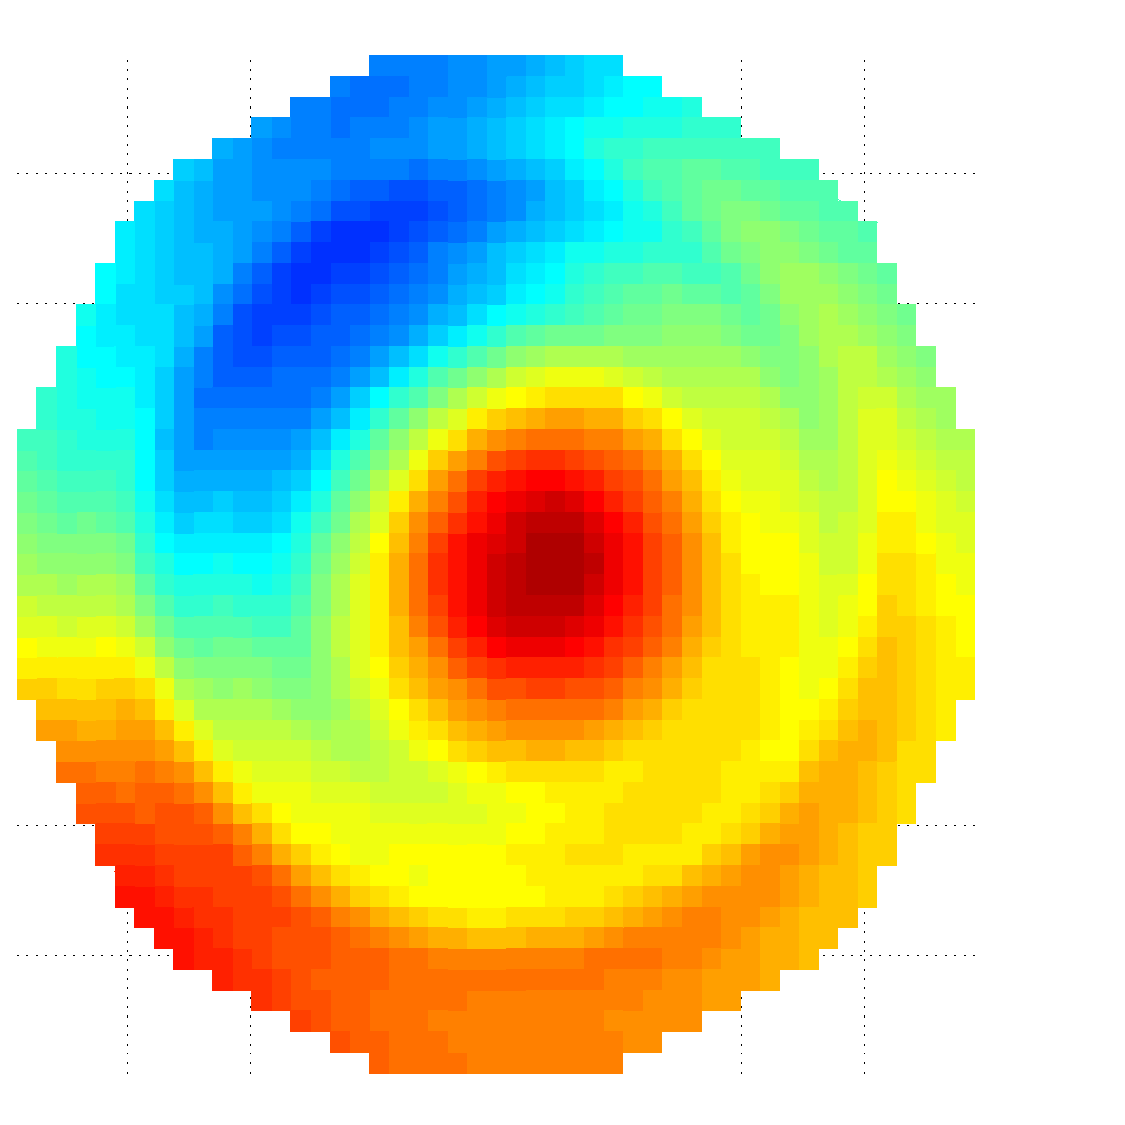
\includegraphics[width=0.4\linewidth]{include/assets/wafer-qoi-true.pdf}
    \flabel{wafer-qoi-true}
  }
  \subfloat[Inferred QoI.]{
    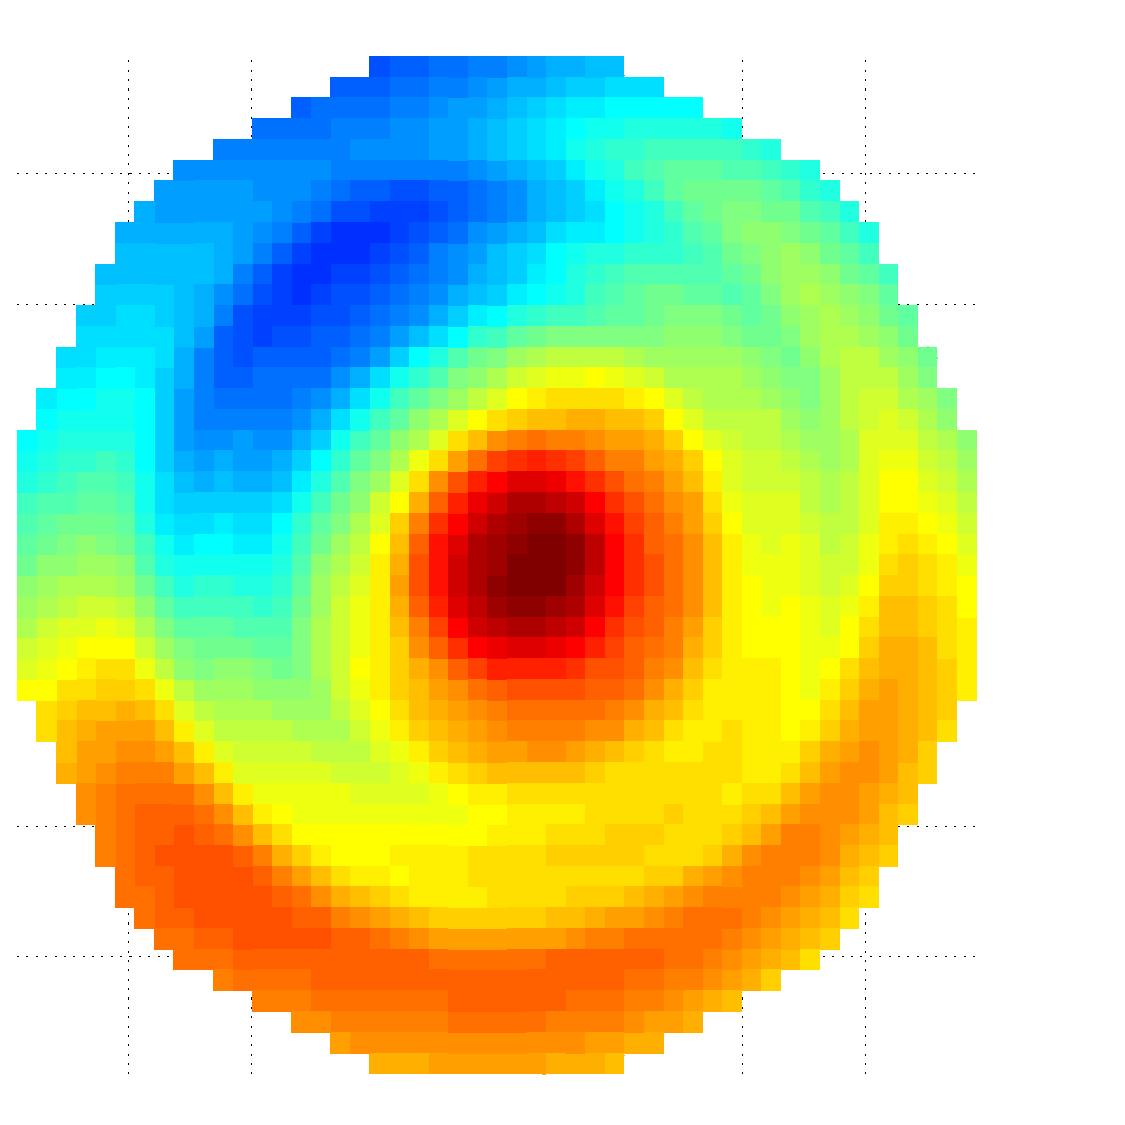
\includegraphics[width=0.4\linewidth]{include/assets/wafer-qoi-inferred.pdf}
    \flabel{wafer-qoi-inferred}
  }
  \caption{The distribution of the QoI across the wafer.}
\end{figure}

Let us consider an example that illustrates an important application of the proposed technique. As previously mentioned, due to process variation, the key parameters that have direct impacts on power and temperature are intrinsically uncertain. Let $\u$ be one of such uncertain quantities; say, the effective channel length.
Assume the technological process imposes a lower bound $\u_*$ on $\u$. This bound separates defective dies ($\u < \u_*$) from those that function properly ($\u_* \leq \u$).
In order to reduce costs, the manufacturer is interested in detecting the faulty dies and taking them out of the production pipeline at early stages. Then, the possible actions that they might take with respect to a single die on the wafer are: (a) keep the die if it closely conforms to the specification; (b) recycle the die, otherwise.
Let the distribution of $\u$ across the wafer be the one depicted on the left side of \fref{wafer-qoi} where the gradient from navy to dark red represents the transition of $\u$ from low to high values.\footnote{The experimental setup is described in detail in \sref{experimental-results}.}
A common approach to find this distribution is to deploy adequate test structures on the dies and measure $\u$ directly; then, an appropriate decision can be taken using the collected information. The problem in this scenario, however, is that the described procedure is technologically complex and, thus, might significantly increase the production costs.

The technique developed in this paper works differently. We apply a fixed workload to a small number of dies on the wafer and measure the corresponding temperature profiles. These profiles can be coarse (low frequency of sampling) and can potentially be corrupted by the measurement noise. Since temperature is cheap to track using, \eg, infrared cameras and no on-die test structures are required, our approach can considerably decrease the costs associated with the characterization of process variation and further decision making.
The result of our framework applied to a data set with less than $7\%$ of the dies on the wafer is shown on the right side of \fref{wafer-qoi}. It can be seen that the two fields closely match each other.

The proposed framework can readily be utilized to estimate probabilities of various events, \eg, $\probabilityMeasure(\u < \u_*)$. This fact is important since, in reality, we do not know the true values and, therefore, can reason about our decisions only in terms of probabilities. We can then reformulate the decision rule defined earlier as follows: (a) keep the die if $\probabilityMeasure(\u_* \leq \u)$ is larger than a certain threshold; (b) recycle the die, otherwise.
An illustration of this rule is given in \fref{wafer-defect} where the threshold is set to two standard deviation below the mean value of $\u$, the crosses mark defective dies (the navy areas in \fref{wafer-qoi}), and the gradient from light gray to red corresponds to the inferred probability of a die to be defective. It can be seen that the inference accurately detects faulty regions.
\begin{figure}[t!]
  \centering
  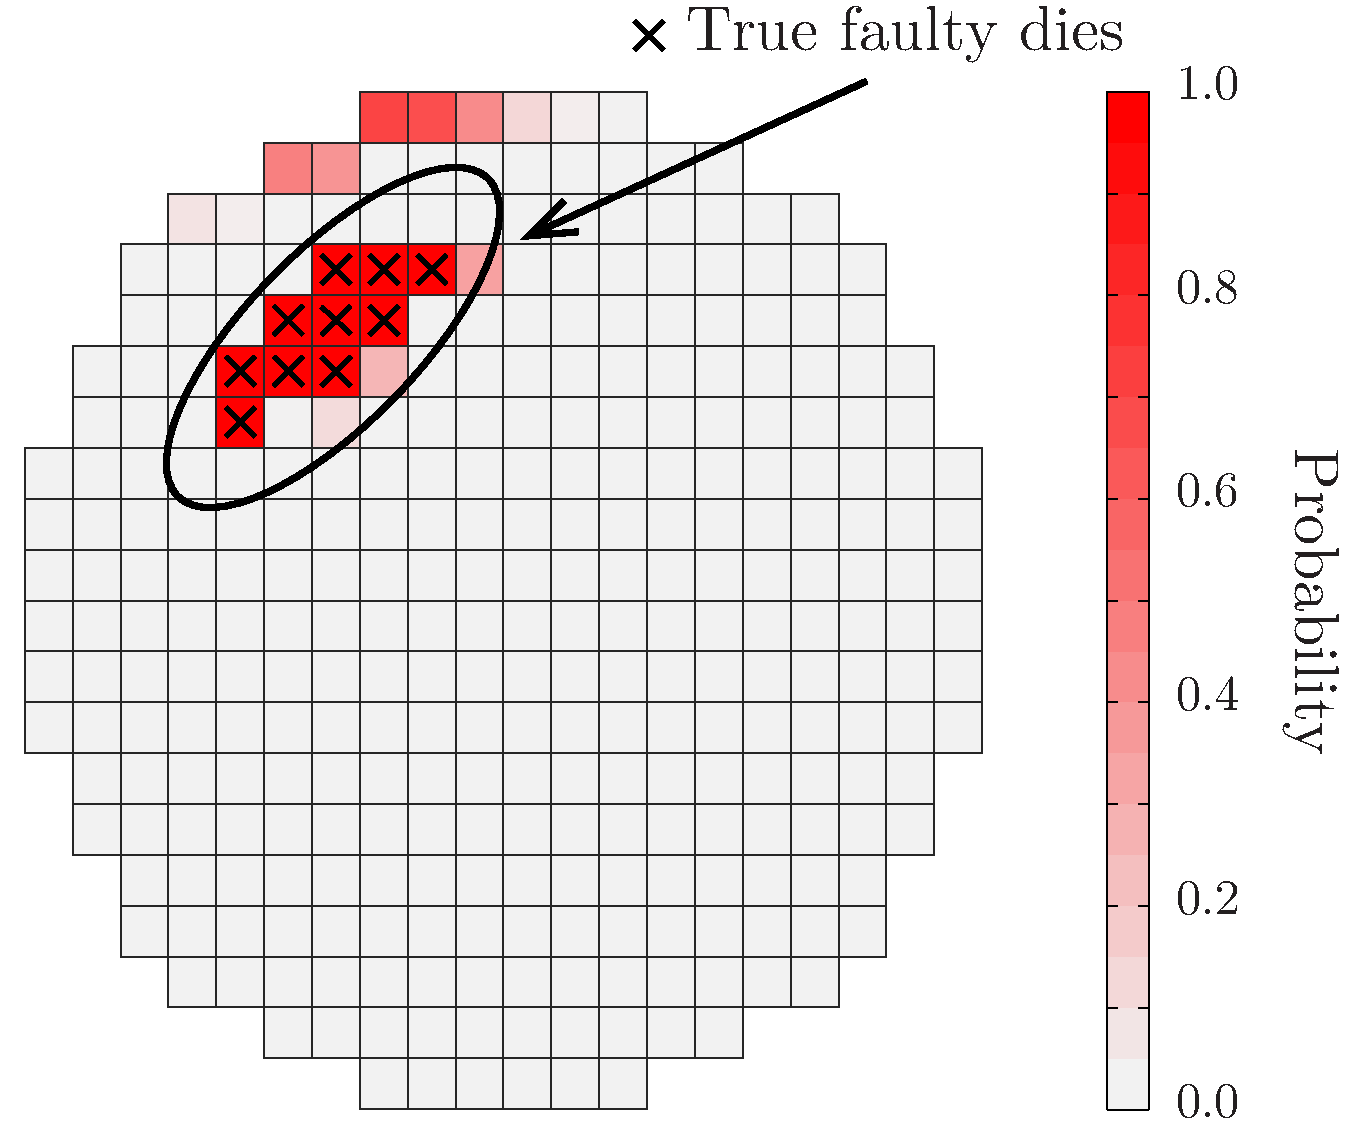
\includegraphics[width=0.6\linewidth]{include/figures/wafer-defect.pdf}
  \caption{Inferred probability of defective dies.}
  \flabel{wafer-defect}
  \vspace{-1.5em}
\end{figure}


In addition, we can introduce a trade-off action: (c) expose the die to a thorough inspection (\eg, via a test structure) if $\probabilityMeasure(\u_* \leq \u)$ is smaller than the threshold of (a) and is larger than some other threshold. In this case, we can reduce costs by examining only those dies for which there is no strong evidence of their satisfactory or unsatisfactory condition.
Furthermore, one can introduce in the inference a so-called utility function, which, for each combination of an outcome of $\u$ and a taken action, assigns the corresponding amount of gain that the decision maker obtains. Then, the inference path, taken in this paper (Bayesian inference), can lead to such an action that maximized the expected utility with respect to the posterior distribution of $\u$. In other words, all possible outcomes of $\u$ weighted by their probabilities will be taken into account in our final decision.
